%interno poro�ilo
%\documentclass[internal, slovene]{FRIreport}

%zaklju�no poro�ilo
%\documentclass[slovene]{FRIreport}

%seminarska naloga
\documentclass[seminar, slovene]{FRIreport}

% AMS fonts required
\usepackage{iopams}  

% package to include graphics in ps, eps or png format
\usepackage{graphicx}
\usepackage{epstopdf}
% the graphics path
\graphicspath{{img/}}

% define equation referencing
\newcommand{\eqref}[1]{(\ref{#1})}

% define figure referencing
\newcommand{\figref}[1]{\ref{#1}}

% define real numbers symbol
\newcommand{\Rset}{\ensuremath{\mathbb{R}}} 
\newcommand{\R}{\Rset} 
% define natural numbers symbol
\newcommand{\Nset}{\ensuremath{\mathbb{N}}} 
\newcommand{\N}{\Nset} 
% define euclidean vector space symbol
\newcommand{\Eset}{\ensuremath{\mathbb{E}}} 
\newcommand{\E}{\Eset} 

\newcommand{\imp}[1]{{\color{P654M}#1\normalcolor}}

%main
\begin{document}

\title{qdCAD: revolucionarni QCA simulator}

\author[M Mo�kon \etal]{Miha Mo�kon, Primo� Pe�ar, Iztok Lebar Bajec}

\address{Skupina 1}

\begin{abstract}
Kratek povzetek je vedno priporo�ljiv saj omogo�a bralcu hitro o\-ce\-no ali je poro�ilo zanj zanimivo ali ne. Povzetek mora biti napisan tako, da strnjeno opi�e vsebino in hkrati posku�a pritegniti bralca. 

\Keywords{kvantni celi�ni avtomat, modeliranje in simulacija}
\end{abstract}



%
%%
\section{Uvod}
%
QCADesigner \cite{walus:2004}, ... troji�ka logika na osnovi troji�kih kvantnih celi�nih avtomatov \cite{lebar_bajec:2005c,lebar_bajec:2006a,lebar_bajec:2006b}.

%
%%
\section{Metode}
%
predstavi uporabljene metode

%
%%
\subsection{Metoda 1}
%
groba predstavitev metode
 
%
%%
\section{Rezultati}
%
prika�i rezultate z uporabo slik ali grafov kot na sliki \figref{fig.Df} in jih obrazlo�i
%
\begin{figure}[htb]
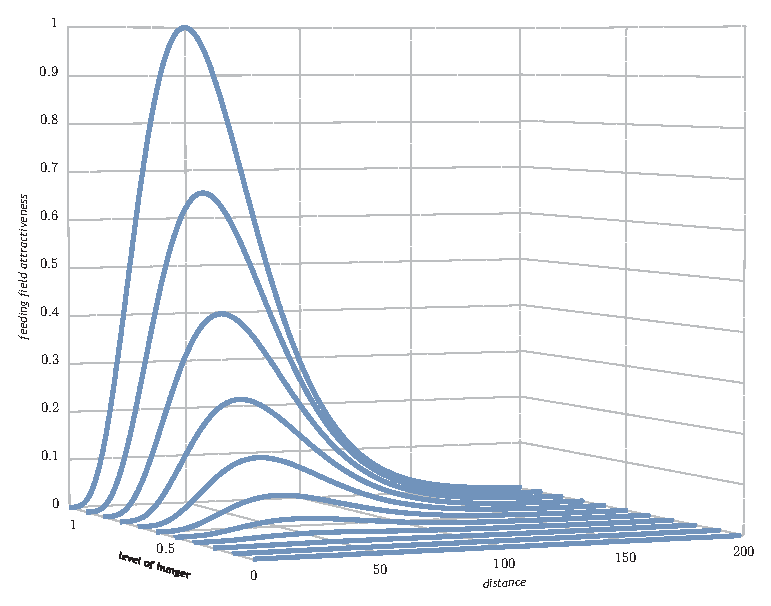
\includegraphics{figDf.eps}
\caption{Uporabi slike za prikaz rezultatov.}
\label{fig.Df}
\end{figure}
%

%
%%
\section{Zaklju�ek}
%
zaklju�i z nekaj izhodi��i za nadaljnje delo

%
%%
\References
%
\bibliographystyle{elsart-num-sl}
%
\bibliography{sample}

\end{document}
